\section{Introduction}

Reinforcement learning for large language model is moving beyond short, single-step tasks toward agentic settings~\citep{prorlagent2026,rllm2025} that require sustained interaction with external environments, such as code repositories~\citep{swebench2024,swegym2024}, web browsers~\citep{zhou2023webarena,deng2023mind2web}, and even full operating systems~\citep{xie2024osworld,wang2025opencua}, through iterative tool use~\citep{shao2024deepseekmath,guo2025deepseek,patil2025the}.
These settings often produce long-horizon trajectories with dozens of interaction steps and tens of thousands of tokens.

\begin{figure}[t]
\centering
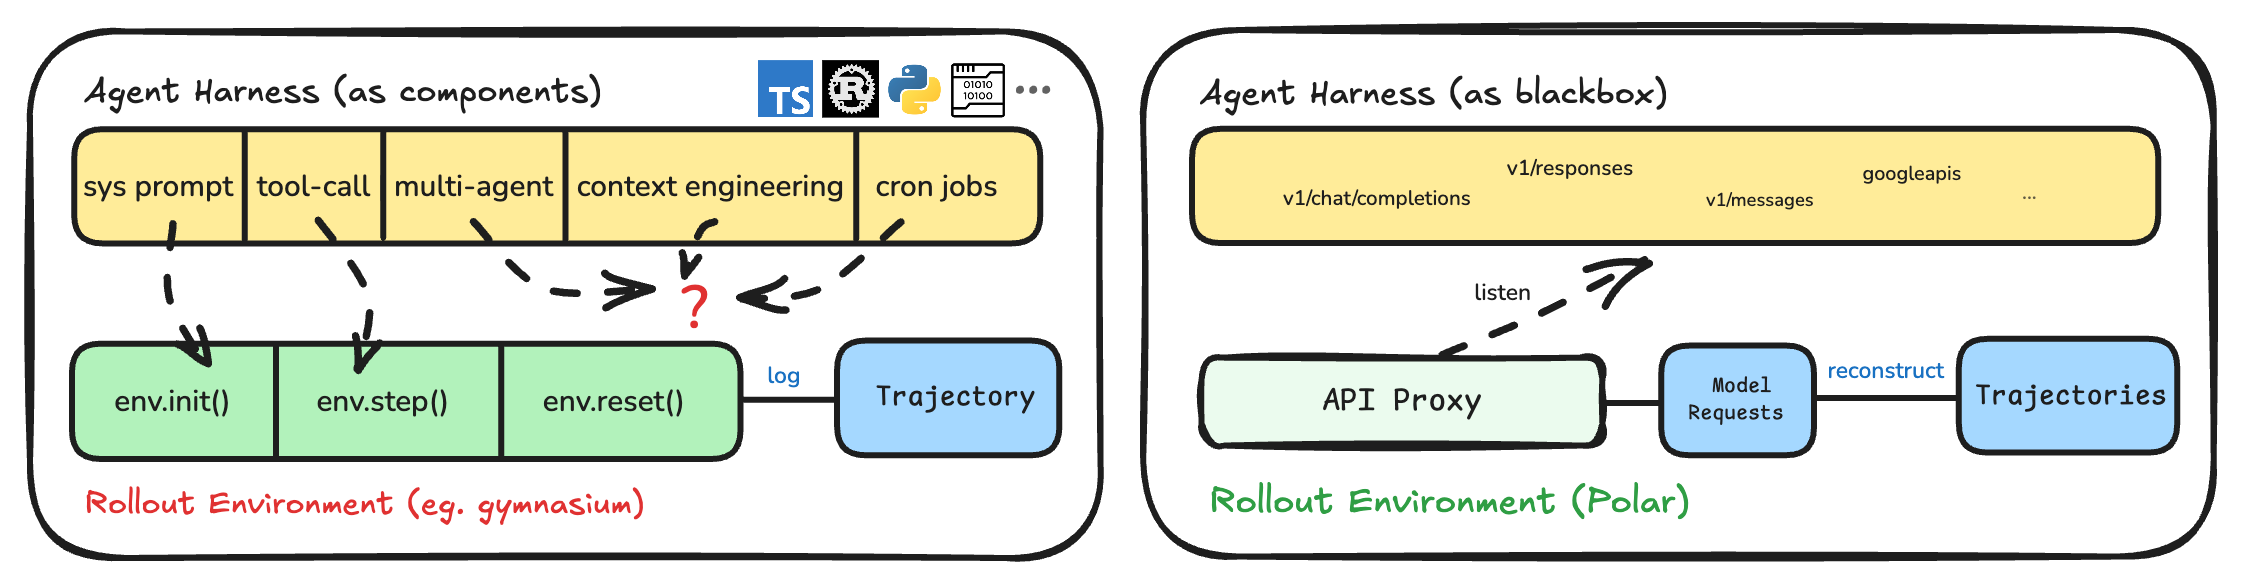
\includegraphics[width=\textwidth]{assets/rollout_style_vs.png}
\caption{\textbf{\polar uses the model API proxy as the rollout boundary.} Traditional rollout frameworks usually require the agent or harness logic to be rewritten behind a framework-owned environment API. This makes the trainer depend on harness-specific integration code and can miss details of the native execution path. \polar instead keeps the harness unchanged and places a provider-compatible proxy at the LLM API boundary; the proxy records prompts, sampled tokens, log probabilities, and responses, then reconstructs trainer-ready trajectories outside the harness.}
\label{fig:rollout_style_comparison}
\end{figure}

This shift makes the training target itself a central systems challenge for agentic RL. Traditional RL often assumes the training target can be exposed through a simple, standardized interface~\citep{brockman2016openai}, allowing researchers to focus mainly on the RL algorithm.
In agentic RL, however, the training target is often a complex software system~\citep{openai_codex_2026, anthropic_claude_code_2026}. It may involve heterogeneous environments~\citep{nemo-gym}, various external tools~\citep{zhang2026nemotronresearchtooln,zhang2024offline}, and long-running workflows~\citep{swebench2024}, and may be implemented in different languages or even distributed as a closed-source binary~\citep{anthropic_claude_code_2026}.

This creates substantial integration burdens. For example, in building agentic RL systems, SkyRL-Agent~\citep{skyrlagent2025} and PRIME-RL~\citep{primerl2026} integrate agent execution directly into the RL pipeline, requiring users to adapt their agents to the RL infrastructure rather than allowing the infrastructure to accommodate existing agent implementations.
This makes the design less flexible: every new agent or harness often requires one framework-specific integration.
Some recent systems attempt to make this integration less intrusive. For instance, Agent Lightning~\citep{agentlightning2025} and rLLM~\citep{rllm2025} reduce this burden by introducing standard tracing interfaces and LLM-call capture mechanisms, but still require agents to conform to prescribed interfaces. Thus, these systems lower the cost of integration but do not fully eliminate it.
These issues are likely to become more severe as agent harnesses grow increasingly complex and, in some cases, even do not expose their internal implementation, making conventional RL integration difficult or even infeasible. Motivated by
these issues, we explore the following central question:

\begin{center}
    \emph{Can we train agents with RL without opening the box?}
\end{center}

That is, without touching their harnesses or forcing them to conform to an RL framework.
The key observation is that, although agents differ widely in their internal implementations, every LLM-based agent must talk to a model. This model API boundary provides a common interface that exists outside the agent itself.
Instead of integrating with the agent harness, we can train by listening to the agent’s LLM calls: capturing its prompts, sampled tokens, log probabilities, and responses, and converting them into RL trajectories. In this view, an agent can be treated as a black box while still becoming trainable.

Building on this intuition, we present \polar: an agentic RL infrastructure that could train \textbf{any} agents as black boxes. The name \polar reflects both its roots in \textbf{P}r\textbf{O}r\textbf{L} \textbf{A}gent serv\textbf{R}~\citep{prorlagent2026} and its role in connecting the two ``poles'' of agent training and deployment: the training environment and the product harness. Instead of treating the agent harness as the RL interface, \polar uses the agent’s LLM API traffic as the interface. Through listening to its model calls through a proxy and converts them into trajectories and rewards for training, the agent runs unchanged.

In addition, \polar separates runtime setup, agent execution, trajectory reconstruction, evaluation, and trainer callbacks behind asynchronous service boundaries. This allows slow and long-tail agent rollouts to scale independently from GPU training, exposing a trainer-agnostic rollout-as-a-service interface for scaling efficient RL infrastructures~\citep{prorlagent2026}.
In summary, the main contributions of this work are:
\begin{itemize}
    \item \textbf{Proxy based rollout and reconstruction over agent harnesses.}
    We propose a paradigm using the agent's LLM API payloads as the RL rollout interface, allowing existing harnesses to serve directly as RL environments without internal code change.
    
    \item \textbf{Rollout-as-a-service architecture for scaling RL infrastructures.}
    \polar separates task submission, runtime setup, harness execution, trajectory reconstruction, evaluation, and trainer callbacks behind asynchronous service boundaries, natively scaling with modern RL infrastructures.

    \item \textbf{Token-faithful trajectory reconstruction.}
    \polar converts raw model requests into token-faithful traces for training. We provide conservative per-request reconstruction and prefix merging for heavy rolllouts, while leaving registry-based extensible interfaces.

    \item \textbf{End-to-end validation on real-world coding harnesses.}
    We validate \polar with RL training on various popular harnesses for software-engineering tasks, and further demonstrate offline SFT data generation with a custom coding harness.
\end{itemize}
